\essaysetup{Strengths and Limits of Formalisation: CW complexes as an example}{Hannah Scholz}

%colors for lean syntax
\definecolor{keywordcolor}{rgb}{0.7, 0.1, 0.1}   % red
\definecolor{tacticcolor}{rgb}{0.0, 0.1, 0.6}    % blue
\definecolor{commentcolor}{rgb}{0.4, 0.4, 0.4}   % grey
\definecolor{symbolcolor}{rgb}{0.0, 0.1, 0.6}    % blue
\definecolor{sortcolor}{rgb}{0.1, 0.5, 0.1}      % green
\definecolor{attributecolor}{rgb}{0.7, 0.1, 0.1} % red


% In your essay, you can use the standard environments. 
% For mathematically-named boxes, we offer in english/german boxes for: remark/bemerkung, theorem/theorem, theorem/satz, proposition/proposition, example/beispiel, corollary/korollar, definition/definition, conjecture/vermutung, lemma/lemma, assertion/behauptung (just the word uses the counter, adding a * does not assign a number to the box), the proof environment works as usual. 
% There is no requirement to use boxes for everything, or even at all! Your text may be free-flowing. 
% Put your essay text here:

Mathematical formalisation is an area of mathematics that has seen exponential growth in the last few years. Simplified, formalisation is the practice of writing a proof in a programming language and then using the computer to verify the validity of the argument. 

Essentially, this works because a proof that A implies B can be seen as a function that sends a proof of A to a proof of B. So when you write a proof of ``A implies B'' in a programming language, you are specifying such a function. Checking the validity of the proof then corresponds to checking that this function indeed sends proofs of A to proofs of B. This correspondence between proofs and programs is called the Curry-Howard isomorphism.

With the advent of powerful AI tools, formalisation has come to be seen as a magic tool that can lend absolute credibility to anyone using it. Every day we see new claims of solutions to previously unsolved problems supposedly backed by formalisation. Therefore, it is critical that we understand what formalisation can actually be helpful with and where it's limits lie. 

This is the focus of the following essay. I will explore this topic with my formalisation of CW complexes in the language Lean as an example. This text assumes no prior knowledge of formalisation or CW complexes. However, I will not explain basic terms from topology but the text should still be understandable without knowing them. This essay is heavily inspired by the essay ``Why formalize mathematics?'' written by Patrick Massot \cite{Massot2021WhyFM}. So if this topic interests you, please check out that essay as well!

\subsection*{What is a CW complexes?}

CW complexes are an important classes of spaces from the area of topology. Their importance is owed to the fact that they are very general spaces that at the same time allow for very powerful results. Intuitively, a CW complex is the result of glueing $n$-cells together along their edges where an $n$-cell is a continuous image of an $n$-disc. You can see examples of $n$-cells of different dimensions in Figure \ref{hannah:scholz:fig:1}.


\begin{figure}[h!]
    \centering
    \begin{minipage}[b]{0.25\linewidth}
            \centering
            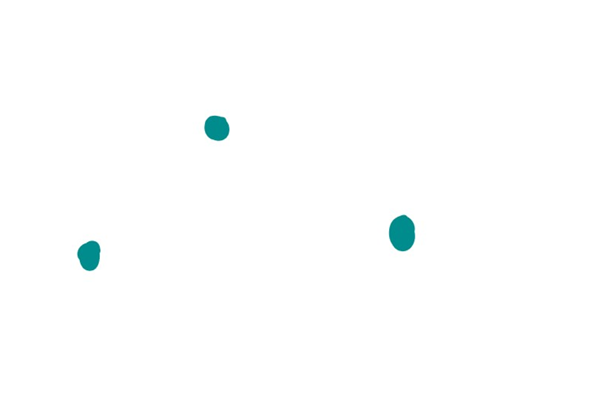
\includegraphics[width=\textwidth]{images/HannahScholzzerocells.png}
        \end{minipage}
        \hspace{0.5cm}
        \begin{minipage}[b]{0.25\linewidth}
            \centering
            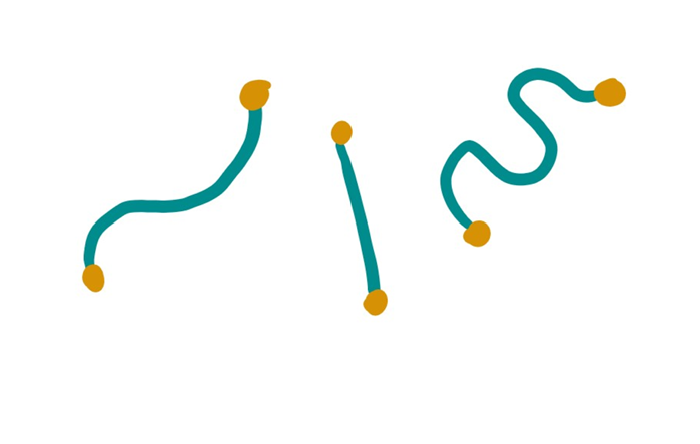
\includegraphics[width=\textwidth]{images/HannahScholzonecells.png}
        \end{minipage}
        \hspace{0.5cm}
        \begin{minipage}[b]{0.25\linewidth}
            \centering
            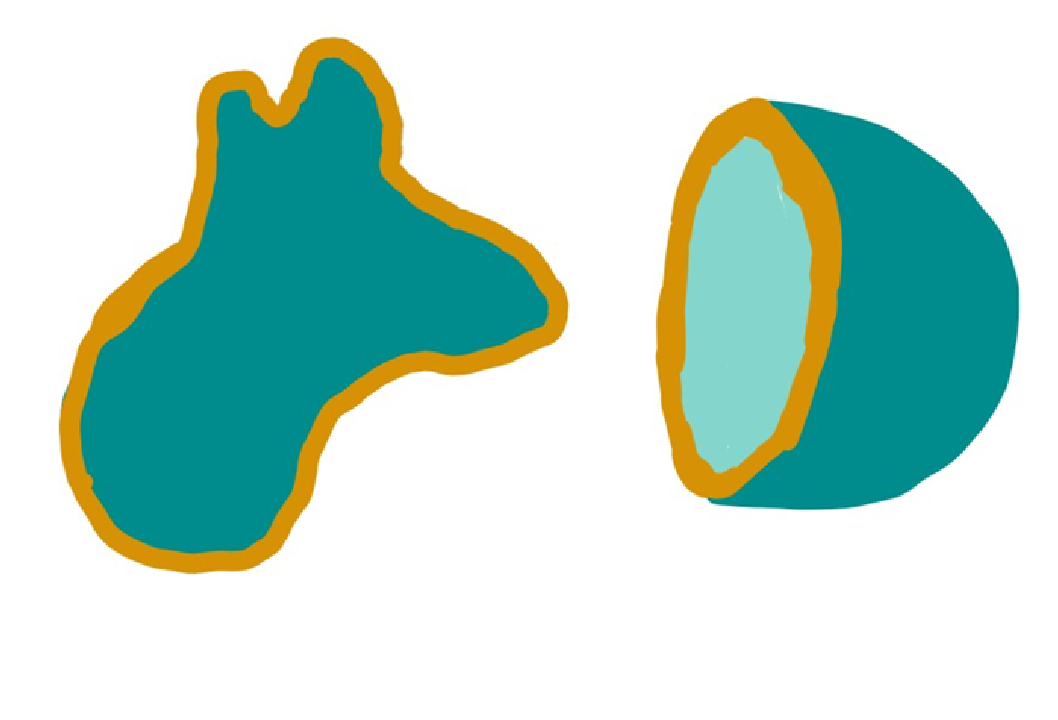
\includegraphics[width=\textwidth]{images/HannahScholztwocells.png}
    \end{minipage}
    \caption{$0$-, $1$- and $2$-cells.}
    \label{hannah:scholz:fig:1}
\end{figure}

By gluing these cells together you can build a lot of the spaces that you already know. In Figure \ref{hannah:scholz:fig:2}, you can see that intervals, the real line and spheres are all CW complexes.

\begin{figure}[h!]
    \centering
    \begin{minipage}[b]{0.25\linewidth}
        \centering
        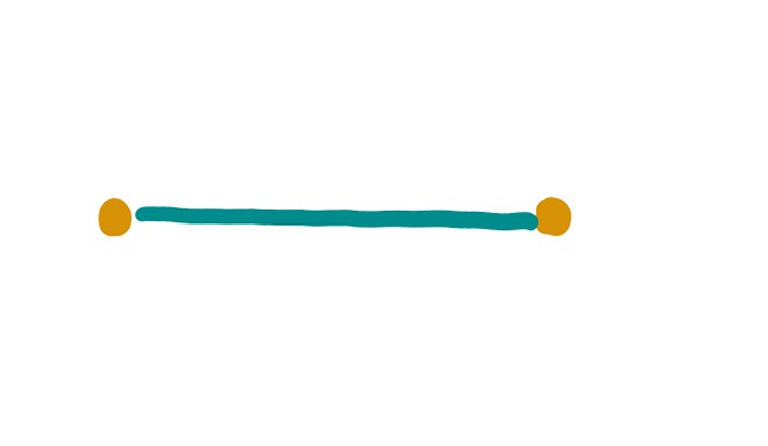
\includegraphics[width=\textwidth]{images/HannahScholzinterval.png}
    \end{minipage}
    \hspace{0.5cm}
    \begin{minipage}[b]{0.5\linewidth}
        \centering
        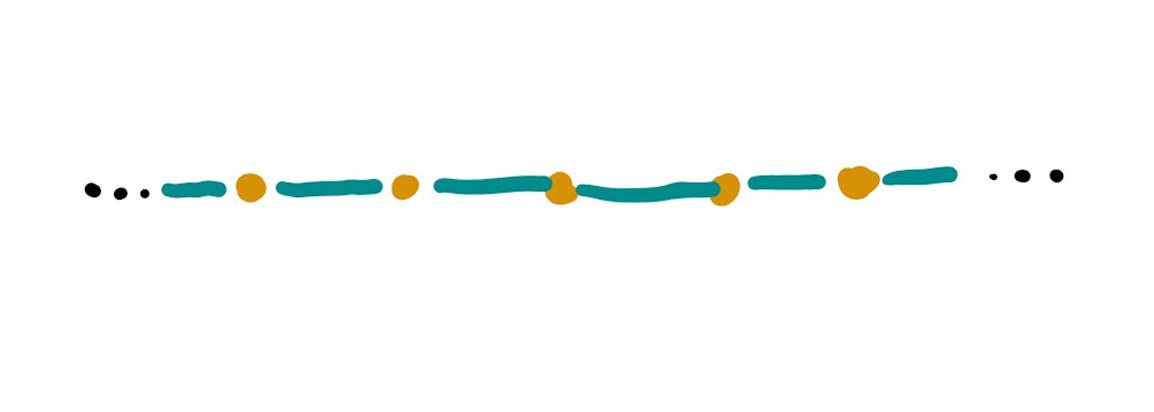
\includegraphics[width=\textwidth]{images/HannahScholzrealline.png}
    \end{minipage}
    %\hspace{0.5cm}
    
\includegraphics[width=0.4\textwidth]{images/HannahScholzsphere.png}
    \caption{CW structures on the interval, real line and two structures on the $2$-sphere.}
    \label{hannah:scholz:fig:2}
\end{figure}

Now we should move from this intuition to the concrete definition. I know, it looks very long and scary but don't worry: I will offer an intuitive explanation below and you don't need to understand all of the details. 

\begin{definition}
Let $X$ be a Hausdorff space. 
An \emph{(absolute) CW complex} on $X$ consists of a family of indexing sets $(I_n)_{n \in \N}$ and a family of continuous maps $(Q_i^n \colon D^n \to X)_{n \in \N, i \in I_n}$ called \emph{characteristic maps} with the following properties: 
\begin{enumerate}[(i)]
    \item $\restrict{Q_i^n}{\interior{D^n}} \colon \interior{D^n} \to Q_i^n(\interior{D^n})$ is a homeomorphism for every $n \in \N$ and $i \in I_n$. We call $\openCell{n}{i} \coloneq Q_i^n(\interior{D^n})$ an \emph{(open) $n$-cell} and $\closedCell{n}{i} \coloneq Q_i^n(D^n)$ a \emph{closed $n$-cell}. \label{hannah:scholz:3}
    \item Two different open cells are disjoint.
    \item For each $n \in \N$ and $i \in I_n$ the \emph{cell frontier} $\cellFrontier{n}{i} \coloneq Q_i^n(\boundary D^n)$ is contained in the union of a finite number of closed cells of a lower dimension. \label{hannah:scholz:4}
    \item A set $A \subseteq X$ is closed if the intersections $A \cap \closedCell{n}{i}$ are closed for all $n \in \N$ and $i \in I_n$. \label{hannah:scholz:5}
    \item The union of all closed cells is $X$. \label{hannah:scholz:6}
\end{enumerate}
\end{definition}

Here $D^n$ refers to the closed unit $n$-disc. The convention for what the symbol $D$ means is different in topology to other fields of mathematics. 

Now for a short explanation: property \ref{hannah:scholz:3} tells you that the open disk needs to be deformed in a reasonable way (e.g.\ no ripping or gluing). Note that the notation for the closed $n$-cell $\closedCell{n}{i}$ is very confusing: it looks like the closed cell is the closure of the open cell but this in not the case in general. Property \ref{hannah:scholz:4} is called ``closure finiteness'' (which is the ``C'' in ``CW complex''). It tells you that the cell frontier needs to be glued to cells of lower dimension and the new cell cannot stretch over infinitely many lower cells. Again, the notation for the cell frontier is confusing: it is not generally the frontier of the open cell. The ``W'' in ``CW complex'' stands for ``weak topology''. This is Property \ref{hannah:scholz:5}. It tells you that the topology on $X$ is determined by the cells. Lastly, Property \ref{hannah:scholz:6} tells you that the whole space is made up of the cells. 

\begin{strength}
    Definitions and notation are unambiguous. 
\end{strength}

% Use boxes for strengths and limits in the color of the Theorem boxes

%\subsection*{Why do we care about CW complexes?}

%CW complexes are an important classes of spaces from the area of topology. Their importance is owed to the fact that they are very general spaces that at the same time allow for very powerful results. Most of the basic topological spaces you know are CW complexes: for example powers of the real numbers $\R^n$ and the complex numbers $\C$, spheres $S^n$, and real projective spaces $\R P^n$ and complex projective spaces $\C P^n$. Then what spaces are not CW complexes? One example is the Hawaiian earring which you can see in Figure \ref{hannah:scholz:fig:1}. They are made up of countably infinite many circles that get smaller and smaller. Intuitively, this isn't a CW complex because there are too many thinks too close together. So as you can see, you need to think of something fairly weird to find a space that isn't a CW complex.

%\begin{figure}
%    \centering
%    \includegraphics[width=.3\textwidth]{images/HannahScholzHawaiianEarring.png}
%    \caption{The Hawaiian earring. This isn't a CW complex.}
%    \label{hannah:scholz:fig:1}
%\end{figure}

% To cite something, write \cite{keyword} and create a .bib-file in which you put your references. Name it yourname.bib. As soon as you cite something, remove the % of the following line and change the "yourname" in the command to your bibliography file name. A very short example is the lib.bib.

\putbib[essays/HannahScholz]

% If you use \label for environments please use the following format: \label {first:last:type:number}: 

%              Example: \label{manuel:hinz:fig:1}

\authorblurb{Here, you can write a few(!) third-person sentences about yourself, your interests and if you want to, a link to your website or similar. If you don't want a blurb to appear, put a \% before the command (without the backslash).}


% If you need additional packages / commands, please say so here:
%
% I added the following lines to the bottom of the myevan.sty file:
%
% Für Lean Code
% \usepackage{listings}
% \def\lstlanguagefiles{lstlean.tex}




